\scanpage{33}\mspage{32.}
% R3 independent proposal. Doubts concern reading and, where indicated, revision state.
% @ top, 1°)
\deleted{\unsure{R|P|Or}} 1°) $F\setminus G\subset F'\setminus G'$ i.e. Tout $A\in F\setminus G$ est $\notin G'$. En effet, si on avait $A\in G'$, on aurait $|A|\subset|G'|=|G|$ donc \deleted{$A\in$} (comme $G\leq F$) $A\in G$.

% @ left margin. Written sideways; the long curve separates it from the body.
\margin{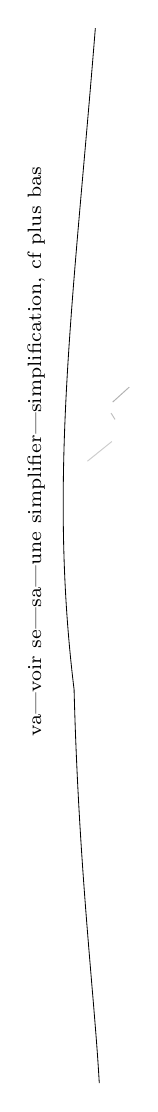
\begin{tikzpicture}[x=1cm,y=1cm]
  \node[rotate=90,anchor=west,inner sep=0pt,font=\scriptsize] at (0,-8.8)
    {\unsure{va|voir} \unsure{se|sa|une} \unsure{simplifier|simplification}, cf plus bas};
  \draw[line width=.3pt] (.75,.2) .. controls (.48,-3.2) and (.15,-5.5) .. (.48,-8.2)
    .. controls (.54,-10.5) and (.74,-12.1) .. (.80,-13.2);
  % Two very faint nonalphabetic stroke clusters immediately right of the rule.
  \draw[black!30,line width=.35pt] (.97,-4.55)--(1.18,-4.36);
  \draw[black!25,line width=.35pt] (.95,-4.69)--(1.00,-4.77);
  \draw[black!20,line width=.35pt] (.65,-5.30)--(.96,-5.05);
\end{tikzpicture}}

% @ upper middle, 2°)
2°) $F'\setminus G'\subset F\setminus G$ Soit $A'\in F'\setminus G'$, prouvons $A'\in F\setminus G$, et d'abord $A'\in F$. \deleted{On a} Soit $A$ le plus petit él. de $F^{A'}$ donc
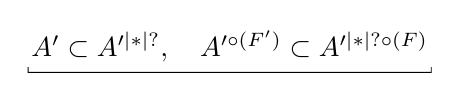
\begin{tikzpicture}[baseline=(bounded.base)]
  \node[inner sep=1pt] (bounded) {$A'\subset A^{\deleted{\unsure{\prime|\ast|?}}},\quad A'^{\circ(F')}\subset A^{\deleted{\unsure{\prime|\ast|?}}\circ(F\unsure{)}}$};
  \draw[line width=.3pt] ([yshift=-.15ex]bounded.south west)--++(0,-.45ex)
    --([yshift=-.6ex]bounded.south east)--++(0,.45ex);
\end{tikzpicture}
% The final closing parenthesis in the rightmost superscript is clipped/indistinct.
% In the next relation, an old membership sign overwritten toward equality is possible,
% but the final state of the curved connector and short middle bar is not secure.
prouvons que $A'\unsure{\in|=}A$ (d'où $A\in F$). \deleted{\unsure{On a|Or}}

% @ middle, Je dis
Je dis que $A\in F\setminus G$ i.e. $A\notin G$, sinon on aurait $A\subset|G|=|G'|$ donc $A'\in G'$ puisque $A'\in F'$ et $G'\leq F'$, absurde. \deleted{Mais} Donc $A\in F\setminus G$, donc $A\in F'$, \deleted{et} Il en résulte que $A^{\circ(F)}=A^{\circ(F')}$ (car $F'\preceq F$
\inserted{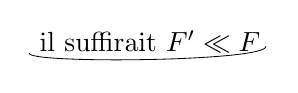
\begin{tikzpicture}[baseline=(suff.base)]
  \node[inner sep=1pt] (suff) {il suffirait $F'\ll F$};
  \draw[line width=.3pt] ([xshift=-.6ex,yshift=.2ex]suff.south west)
    .. controls ([xshift=-.7ex,yshift=-.7ex]suff.south west) and ([xshift=.5ex,yshift=-.5ex]suff.south east)
    .. ([xshift=.2ex,yshift=.8ex]suff.south east);
\end{tikzpicture}}\deleted{)} cf lemme plus bas) et \unsure{\uline{bien}|\deleted{bien}} \deleted{$\unsure{F|\in|\exists}$} $A,A'\in F'$ tels que $A'^{\circ(F')}\subset A^{\circ(F')}$, ce qui prouve $A=A'$.

% @ lower middle, Donc
Donc \unsure{on a} prouvé que $\deleted{\unsure{F|A}}A'\in F'\setminus G'\Rightarrow A'\in F$. Prouvons qu'on a $A'\notin G$ (d'où $A'\in F\setminus G$\deleted{)}, qed). Sinon on aurait $A'\in G$, on aurait $A'\subset |G|=|G'|$, d'où
% @ pale unattached mark just above the following parenthetical line.
\figure{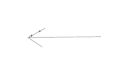
\begin{tikzpicture}[x=.12cm,y=.12cm]
  \draw[black!20,line width=.35pt] (0,0)--(7.7,.1);
  \draw[black!20,line width=.35pt] (1.8,1.0)--(0,0)--(1.5,-1.0);
  \fill[black!55] (1.22,.67) circle (.10);
  \fill[black!60] (.35,.21) circle (.11);
  \fill[black!45] (.13,.04) circle (.07);
\end{tikzpicture}}
(comme $A'\in F'$ et $G'\leq F'$) $A'\in G'$, absurde.

% @ lower third: cancelled b) => c) draft. The actual five diagonal strokes and
% insertion leader are retained; the final Prouvons line lies below their ends.
\figure{\begin{tikzpicture}[x=1cm,y=1cm]
  \node[anchor=west,inner sep=0pt,font=\small] at (3.4,.53)
    {\deleted{\inserted{On suppose b) i.e. $\varphi$ induit $F'\setminus G'\overset{\sim}{\longrightarrow}F\setminus G$}}};
  \node[anchor=west,inner sep=0pt,font=\small] at (0,0)
    {\deleted{b) $\Rightarrow$ c) Soit $A\in F\setminus G$, prouvons que}};
  \node[anchor=west,inner sep=0pt,font=\small] at (0,-.68)
    {\deleted{$A^{\circ(F)}$ est une \uline{strate ouverte \deleted{dans \unsure{la}} de $F'$}. Soit}};
  \node[anchor=west,inner sep=0pt,font=\small] at (0,-1.36)
    {\deleted{$A'\in F'\setminus G'$ l'unique élément \deleted{de} tel que $\varphi(A')=A$.}};
  \draw[line width=.3pt] (3.05,-.05) .. controls (2.70,.32) and (3.35,.34) .. (4.5,.39)
    .. controls (8.0,.65) and (11.5,.52) .. (12.5,.68)
    .. controls (12.85,.72) and (12.84,.88) .. (12.82,.94);
  \draw[line width=.5pt] (1.65,.22)--(.10,-1.63);
  \draw[line width=.5pt] (4.52,.66)--(2.58,-1.68);
  \draw[line width=.5pt] (7.46,.63)--(5.53,-1.64);
  \draw[line width=.5pt] (9.83,.58)--(8.18,-1.62);
  \draw[line width=.5pt] (11.89,.52)--(10.45,-1.54);
\end{tikzpicture}}
% Deletion-state uncertainty, not two successive manuscript occurrences:
\unsure{\deleted{Prouvons $A'^{\circ(F')}=A^{\circ(F)}$.}|Prouvons $A'^{\circ(F')}=A^{\circ(F)}$.}

% @ bottom: new b <=> c argument
b $\Longleftrightarrow$ c \deleted{Posons} On a $|F|\setminus|G|=|F'|\setminus|G'|$, soit $U$, Posons $F\setminus G=I^{\unsure{\ast|k|+}},\ F'\deleted{\unsure{\times|\setminus}}\unsure{\setminus}G'=I'^{\ast}$ (parties ouvertes des ens d'indices ordonnés $I$, \deleted{$\unsure{A|\Delta}$} $(=F)$, $I'(=F')$. On a
